\section{Spørgsmål 2}

\subsection{Fokuspunkter}
\begin{itemize}
	\item Hvorledes omsættes et konceptuelt databasedesign til en konkret database?
	\item Kom bla. ind på begreberne "\textit{designregler}, \textit{relations modellering}, samt \textit{skema}.
\end{itemize}

\subsection{Litteratur}
\begin{itemize}
	\item Kap. 2 fra \textit{Database eLearning} - $http://db.grussell.org/index.html)$
	\begin{itemize}
		\item Database Analysis.
		\item Entity Relationship Modelling.
		\item Mapping ER Models into relations.
		\item Advanced ER Mapping.
	\end{itemize}
	\item Database Modelling and Design
	\begin{itemize}
		\item Kap. 1 (s. 1 - 11).
		\item Kap. 3 (s. 35 - 53).
		\item Kap. 5 (s. 85 - 108).
	\end{itemize}
\end{itemize}

\newpage

% must
\subsection{Hvorledes omsættes et konceptuelt databasedesign til en konkret database?}
Som i objektorientering: finder
betydende klasser i problemdomænet. Analyserer klassernes association, baggrund af disse opstilles en model for den kommende database. Modellen er typisk udført i et Entity Relationship Diagram (ER) eller i et klassediagram (UML).

\begin{enumerate}
	\item Identificer entiteter og deres attributter.
	\item Definer relationer mellem entiteterne.
	\item Anvend De 10 designregler.
\end{enumerate}

En grund til at lave et velovervejet design er at minimere risikoen for anormaliteter, dvs. fejl eller uregelmæssigheder der opstår i data. Her kan også anvendes normalisering\todo{pageref!}, men det er et andet emne.

\subsubsection{Faldgruber}
Når designet laves, er der faldgrupper. Det kan f.eks. være en \textbf{fan trap} eller \textbf{chasm trap}. Disse er kendt som \textbf{Connection Traps} 

\paragraph{Fan trap} opstår, når en entitet har \textit{1:M} relation til mindst to entiteter. På figur~\ref{fig:fan} kan man se at et \textit{Site} har flere \textit{Department} og \textit{Staff}. Problemet bliver så: \textit{''which staff work in a particular department?''}

\begin{figure}[h]
\centering
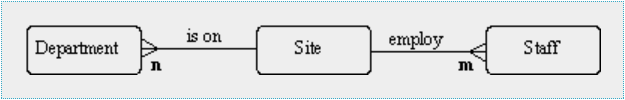
\includegraphics[width=0.8\linewidth]{figs/spm2/fan}
\caption{Fan Trap.}
\label{fig:fan}
\end{figure}

På figur~\ref{fig:fan_solved} vises det hvordan problemet løses ved at ændre ER modellen til at vise den korrekte association.

\begin{figure}[h]
\centering
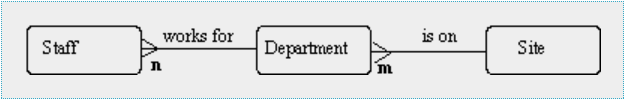
\includegraphics[width=0.8\linewidth]{figs/spm2/fan_solved}
\caption{Fan Trap Resolved.}
\label{fig:fan_solved}
\end{figure}

\paragraph{Chasm trap} 

% must
\subsection{De 10 Designregler}

\begin{enumerate}
	\item \textbf{Entity}\\
	Én entitet skal svare en én tabel. Entiteten skal have samme navn som tabellen. Skal også helst være et navneord i ental. 
	
	\item \textbf{Many-to-many binary relationship}\\
	Entiteternes primærnøgler bliver sammensat i en ny entitet, hvor de er fremmednøgler.
	
	\item \textbf{One-to-many binary relationship}\\
	''Mange''-entiteten skal have fremmednøglen, ellers brydes 1. normalform\todo{le fuq? Indsæt muligvis pageref til andet spm}.
	
	\item \textbf{Recursive binary relationship}\\
	Samme regler er gældende som ved binære relationer.
	
	\item \textbf{Ternary relationship}\\
	En weaktabel oprettes med en primær nøgle der er sammensat af de 3 fremmednøgler.\todo{Slide says ''+other stuff'', what other stuff?}
	
	\item \textbf{Attribute of an entity}\\
	En attribut af en entitet kan mappes direkte som en attribut i entitetens tabel.
	
	\item \textbf{Generalization super-class (super-type) entity}\\
	En super entitet mappes direkte til en SQL tabel.
	
	\item \textbf{Generalization super-class (subtype) entity}\\
	En sub entitet mappes til sin egen table for super entiteten. Primær nøglen fra super entiteten
	bliver fremmednøgle hos sub entiteten.
	
	\item \textbf{Mandatory constrint (1 lower bound) on the “one” side of a one-to-many relationship}\\
	Fremmednøglen skal ligge på mange siden, og sættes til ’not null’. Eks. En video skal ejes af en
	butik, butik behøver ikke eje en video. Ved at sætte fremmednøglen på mange siden får vi at; en
	butik kan godt oprettes uden en video, men en video skal tilknyttes en butik.
	
	\item \textbf{Subject gets targets Primary key as foreign key}\\
	I en 1 til 1 relation skal man identificere subject og target. Target har interesse i subjekt.
	
\end{enumerate}

% must
\subsection{Relationsmodellering}

% must
\subsection{Skema}